\documentclass{article}
\usepackage{graphics,indentfirst,amsmath,amsthm,amssymb,latexsym,enumerate}
\usepackage{graphicx}
\usepackage{zed-csp}
%%%%%%%%%%%%%%%%%%%%%%%%%%%%%%%%%%%%%%%%%%%%%%%%%%%%%%%%%%%%%%%%
%  6.826 (POCS Seminar) macro file for handouts and problem sets.
%
% You should save this file as handout.tex
%
% Your main LaTeX file should look like this:
%
%        \documentstyle[12pt]{article}
%
%        %%%%%%%%%%%%%%%%%%%%%%%%%%%%%%%%%%%%%%%%%%%%%%%%%%%%%%%%%%%%%%%%
%  6.826 (POCS Seminar) macro file for handouts and problem sets.
%
% You should save this file as handout.tex
%
% Your main LaTeX file should look like this:
%
%        \documentstyle[12pt]{article}
%
%        %%%%%%%%%%%%%%%%%%%%%%%%%%%%%%%%%%%%%%%%%%%%%%%%%%%%%%%%%%%%%%%%
%  6.826 (POCS Seminar) macro file for handouts and problem sets.
%
% You should save this file as handout.tex
%
% Your main LaTeX file should look like this:
%
%        \documentstyle[12pt]{article}
%
%        \input{handout}
%%%%%%%%%%%%%%%%%%%%%%%%%%%%%%%%%%%%%%%%%%%%%%%%%%%%%%%%%%%%%%%%

\oddsidemargin 0in
\evensidemargin 0in
\marginparwidth 40pt
\marginparsep 10pt
\topmargin 0pt
\headsep 0in
\headheight 0in
\textheight 8.5in
\textwidth 6in
\brokenpenalty=10000

% \handout{number}{date}{title}

\newcommand{\handout}[3]{


\begin{center}
\rule{\textwidth}{.0075in} \\
\rule[3mm]{\textwidth}{.0075in}\\

CMU 17-651\hfill Models of Software Systems\hfill Fall 2018\\[3ex]

{\Large\bf #3}\\[3ex]

Dario A Lencina-Talarico \hfill {\bf Handout #1} \hfill #2

\rule{\textwidth}{.0075in} \\
\rule[3mm]{\textwidth}{.0075in} \\
\end{center}

}

% \homework{number}{date}{title}{due-date}
\newcommand{\homework}[4]{

\begin{center}
\rule{\textwidth}{.0075in} \\
\rule[3mm]{\textwidth}{.0075in}\\

CMU 17-651\hfill Models of Software Systems\hfill Fall 2018\\[3ex]

{\Large\bf #3} \\[3ex]

Dario A Lencina Talarico \hfill  #1  \hfill Due: #2\\

\rule{\textwidth}{.0075in} \\
\rule[3mm]{\textwidth}{.0075in} \\
\end{center}

%\noindent
%{\bf Due date: #4}

}

% \solutionset{number}{date}{title}{due-date}
\newcommand{\solutionset}[4]{

\begin{center}
\rule{\textwidth}{.0075in} \\
\rule[3mm]{\textwidth}{.0075in}\\

CMU 17-651\hfill Models of Software Systems\hfill Fall 2016\\[3ex]

{\Large\bf #3} \\[3ex]

Garlan  \hfill  Solutions for Homework #1  \hfill  #2\\

\rule{\textwidth}{.0075in} \\
\rule[3mm]{\textwidth}{.0075in} \\
\end{center}

%\noindent
%{\bf Due date: #4}

}

% \problem{problem-number}
\newcommand{\problem}[1]{
\vspace{2ex}
\noindent
{\bf Problem #1.}

}

% \solution{solution-number}{points}
\newcommand{\solution}[2]{
\vspace{3ex}
\noindent
{\bf Problem #1}  (#2 points)

}

\newcommand{\cscomment}{
\vspace{1ex}
\noindent Comments: }

% \parts{part-alphabet}{points}
\newcommand{\parts}[2]{
\vspace{2ex}
\noindent
{\bf (#1)}  (#2 points)

}

% \problems{problems-number}{points}
\newcommand{\problems}[2]{
\vspace{3ex}
\noindent
{\bf Problem #1}  (#2 points)

}

\newenvironment{symbolfootnotes}{\def\thefootnote{\fnsymbol{footnote}}}{}

%%%%%%%%%%%%%%%%%%%%%%%%%%%%%%%%%%%%%%%%%%%%%%%%%%%%%%%%%%%%%%%%

\oddsidemargin 0in
\evensidemargin 0in
\marginparwidth 40pt
\marginparsep 10pt
\topmargin 0pt
\headsep 0in
\headheight 0in
\textheight 8.5in
\textwidth 6in
\brokenpenalty=10000

% \handout{number}{date}{title}

\newcommand{\handout}[3]{


\begin{center}
\rule{\textwidth}{.0075in} \\
\rule[3mm]{\textwidth}{.0075in}\\

CMU 17-651\hfill Models of Software Systems\hfill Fall 2018\\[3ex]

{\Large\bf #3}\\[3ex]

Dario A Lencina-Talarico \hfill {\bf Handout #1} \hfill #2

\rule{\textwidth}{.0075in} \\
\rule[3mm]{\textwidth}{.0075in} \\
\end{center}

}

% \homework{number}{date}{title}{due-date}
\newcommand{\homework}[4]{

\begin{center}
\rule{\textwidth}{.0075in} \\
\rule[3mm]{\textwidth}{.0075in}\\

CMU 17-651\hfill Models of Software Systems\hfill Fall 2018\\[3ex]

{\Large\bf #3} \\[3ex]

Dario A Lencina Talarico \hfill  #1  \hfill Due: #2\\

\rule{\textwidth}{.0075in} \\
\rule[3mm]{\textwidth}{.0075in} \\
\end{center}

%\noindent
%{\bf Due date: #4}

}

% \solutionset{number}{date}{title}{due-date}
\newcommand{\solutionset}[4]{

\begin{center}
\rule{\textwidth}{.0075in} \\
\rule[3mm]{\textwidth}{.0075in}\\

CMU 17-651\hfill Models of Software Systems\hfill Fall 2016\\[3ex]

{\Large\bf #3} \\[3ex]

Garlan  \hfill  Solutions for Homework #1  \hfill  #2\\

\rule{\textwidth}{.0075in} \\
\rule[3mm]{\textwidth}{.0075in} \\
\end{center}

%\noindent
%{\bf Due date: #4}

}

% \problem{problem-number}
\newcommand{\problem}[1]{
\vspace{2ex}
\noindent
{\bf Problem #1.}

}

% \solution{solution-number}{points}
\newcommand{\solution}[2]{
\vspace{3ex}
\noindent
{\bf Problem #1}  (#2 points)

}

\newcommand{\cscomment}{
\vspace{1ex}
\noindent Comments: }

% \parts{part-alphabet}{points}
\newcommand{\parts}[2]{
\vspace{2ex}
\noindent
{\bf (#1)}  (#2 points)

}

% \problems{problems-number}{points}
\newcommand{\problems}[2]{
\vspace{3ex}
\noindent
{\bf Problem #1}  (#2 points)

}

\newenvironment{symbolfootnotes}{\def\thefootnote{\fnsymbol{footnote}}}{}

%%%%%%%%%%%%%%%%%%%%%%%%%%%%%%%%%%%%%%%%%%%%%%%%%%%%%%%%%%%%%%%%

\oddsidemargin 0in
\evensidemargin 0in
\marginparwidth 40pt
\marginparsep 10pt
\topmargin 0pt
\headsep 0in
\headheight 0in
\textheight 8.5in
\textwidth 6in
\brokenpenalty=10000

% \handout{number}{date}{title}

\newcommand{\handout}[3]{


\begin{center}
\rule{\textwidth}{.0075in} \\
\rule[3mm]{\textwidth}{.0075in}\\

CMU 17-651\hfill Models of Software Systems\hfill Fall 2018\\[3ex]

{\Large\bf #3}\\[3ex]

Dario A Lencina-Talarico \hfill {\bf Handout #1} \hfill #2

\rule{\textwidth}{.0075in} \\
\rule[3mm]{\textwidth}{.0075in} \\
\end{center}

}

% \homework{number}{date}{title}{due-date}
\newcommand{\homework}[4]{

\begin{center}
\rule{\textwidth}{.0075in} \\
\rule[3mm]{\textwidth}{.0075in}\\

CMU 17-651\hfill Models of Software Systems\hfill Fall 2018\\[3ex]

{\Large\bf #3} \\[3ex]

Dario A Lencina Talarico \hfill  #1  \hfill Due: #2\\

\rule{\textwidth}{.0075in} \\
\rule[3mm]{\textwidth}{.0075in} \\
\end{center}

%\noindent
%{\bf Due date: #4}

}

% \solutionset{number}{date}{title}{due-date}
\newcommand{\solutionset}[4]{

\begin{center}
\rule{\textwidth}{.0075in} \\
\rule[3mm]{\textwidth}{.0075in}\\

CMU 17-651\hfill Models of Software Systems\hfill Fall 2016\\[3ex]

{\Large\bf #3} \\[3ex]

Garlan  \hfill  Solutions for Homework #1  \hfill  #2\\

\rule{\textwidth}{.0075in} \\
\rule[3mm]{\textwidth}{.0075in} \\
\end{center}

%\noindent
%{\bf Due date: #4}

}

% \problem{problem-number}
\newcommand{\problem}[1]{
\vspace{2ex}
\noindent
{\bf Problem #1.}

}

% \solution{solution-number}{points}
\newcommand{\solution}[2]{
\vspace{3ex}
\noindent
{\bf Problem #1}  (#2 points)

}

\newcommand{\cscomment}{
\vspace{1ex}
\noindent Comments: }

% \parts{part-alphabet}{points}
\newcommand{\parts}[2]{
\vspace{2ex}
\noindent
{\bf (#1)}  (#2 points)

}

% \problems{problems-number}{points}
\newcommand{\problems}[2]{
\vspace{3ex}
\noindent
{\bf Problem #1}  (#2 points)

}

\newenvironment{symbolfootnotes}{\def\thefootnote{\fnsymbol{footnote}}}{}


\begin{document}

\homework{}{1 October 2018}{Homework \#5: State Machines}{}

\begin{enumerate}

\item A certain, simple, answering machine has two buttons, ``play''
and ``save'' and can, of course, receive messages. If someone plays
the messages and doesn't save them, they are erased/overwritten when
the next incoming message is received. The answering machine only
holds a specified number of messages; when it reaches full capacity
it refuses to accept new messages. The answering machine can be
modeled by the state machine, $\mathbf{AnsMachine}$, whose state
transition diagram is attached.

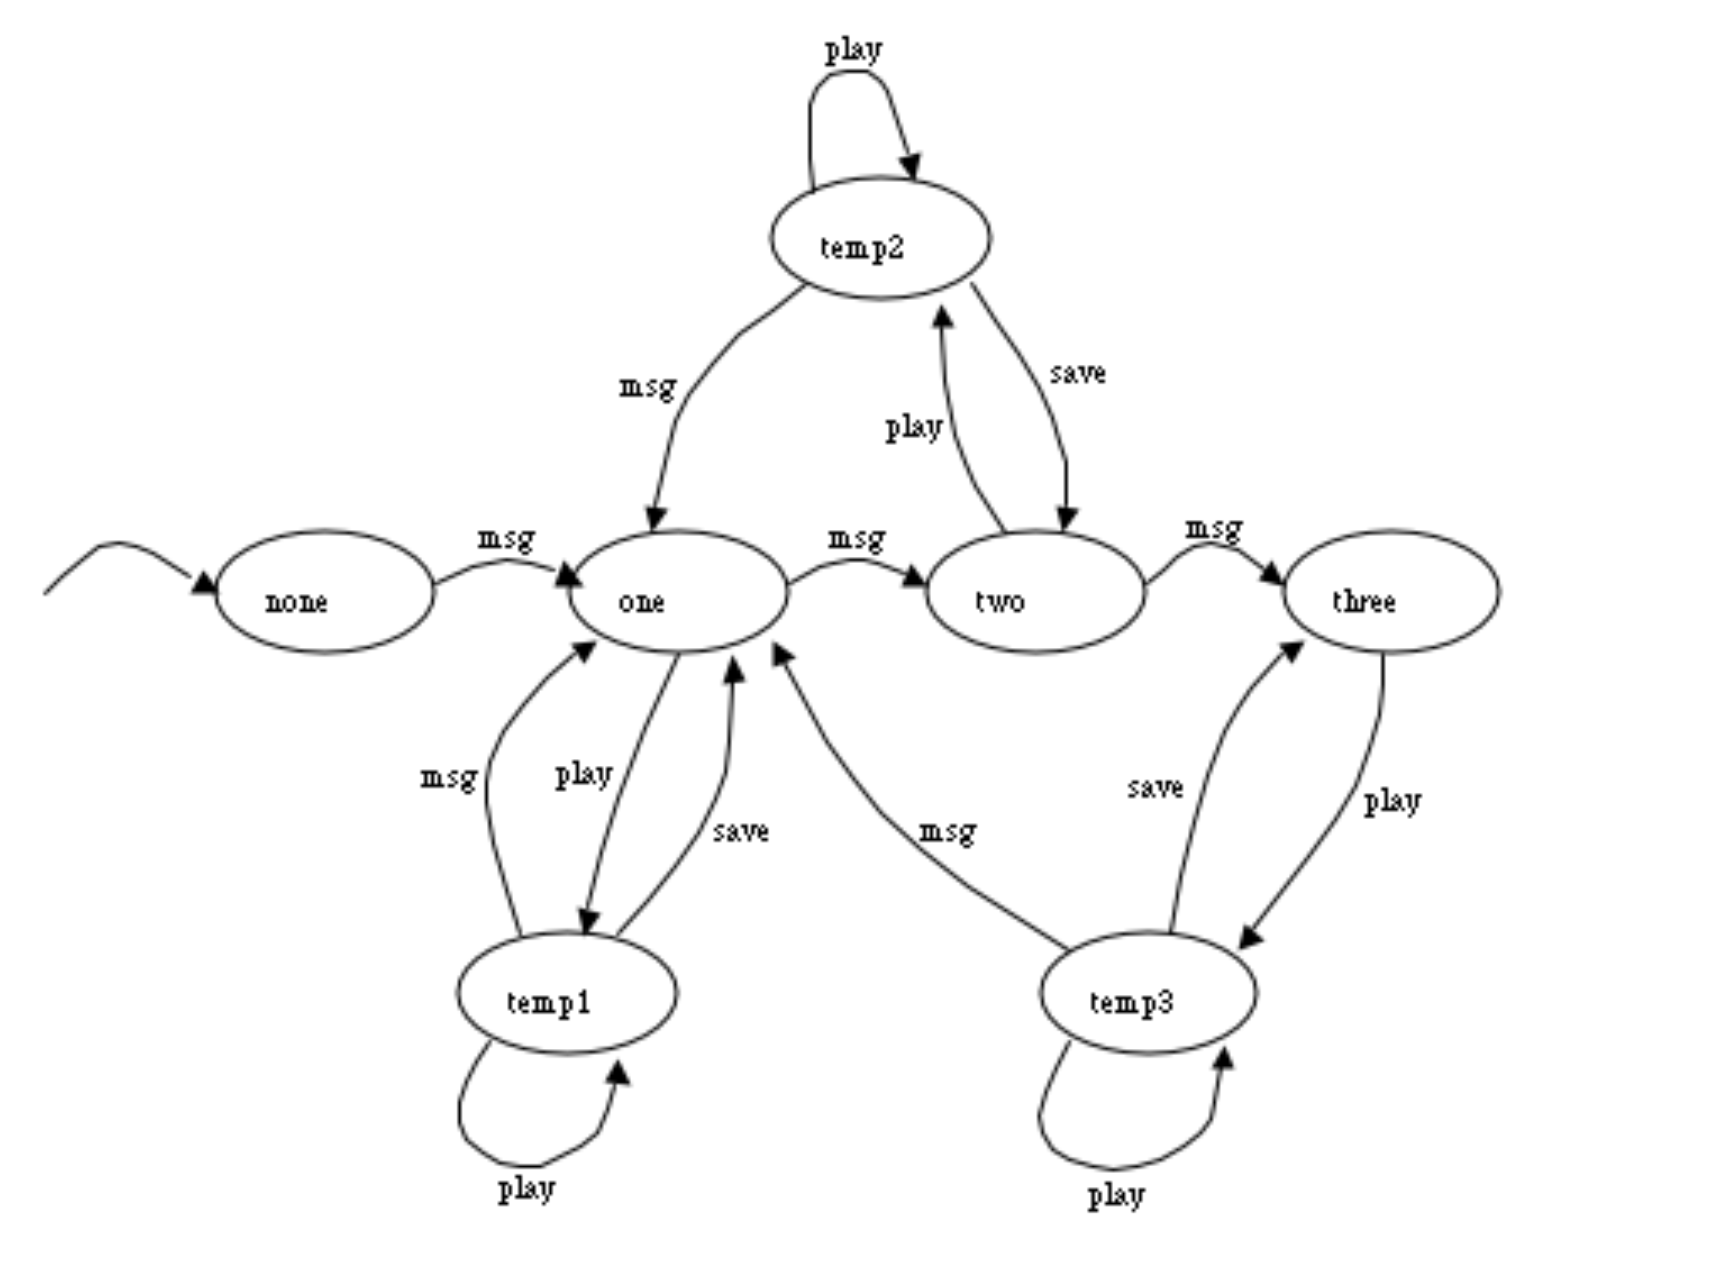
\includegraphics[width=4in]{ansmachine.png}

\begin{enumerate}
 \item Give a 4-tuple description for this state machine. \\
   AnsweringMachine == ( \\
   $\{none,one,two,three,temp1,temp2,temp3 \}$, \\
   $\{none \}$, \\
   $\{msg, play, save \}$, \\
   $\{(none, msg, one),$ \\
   $ (one, msg, two), (one, play, temp1),$ \\
   $ (two, msg, three),(two, play, temp2),$ \\
   $ (temp1, save, one), (temp1, msg, one), (temp1, play, temp1), $ \\
   $ (temp2, save, two), (temp2, play, temp2), (temp2, msg, one),$ \\
   $ (temp3, play, temp3), (temp3, save, tree), temp3, msg, one) \}$ \\
   ) \\
 \item Give three execution fragments of {\bf AnsMachine}, at least one of which is not an
   execution. \\
   Given the GWC10 definition of execution fragment and execution: \\
   ``Definition 3. An execution fragment is a finite or infinite sequence $\langle$ s0,a1,s1,a2,s3,... $\rangle$ of alternating states and actions such that for all i (si,ai+1,si+1) is a step of M.''\\
   \\
   ``Definition 4. An execution is an execution fragment starting with an initial state of M (and ending in a state if finite)'' \\
   \begin{enumerate}
   \item $\langle none, msg, one, play, temp1, msg, one, msg, two \rangle$
   \item $\langle none, msg, one, msg, two, play, temp2, save, two\rangle$
   \item Execution which is not an execution frament: \\ $\langle two, msg, three, play, temp3, play, temp3, msg, one \rangle$ \\
     It is not an execution fragment because it starts at state two as opposed to $none$ \\
   \end{enumerate}
 
 \item Give both a finite and an infinite execution of
   {\bf AnsMachine}.
   \begin{enumerate}
   \item finite == $\langle none, msg, one, play, temp2, save \rangle$
   \item infinite == $\langle none, msg, one, play, temp1, msg, one, play, temp1, ... \rangle$ \\
     I am not sure if I am using the right notation for the infinite execution, since $none$ is not repeated, only the $\{msg, one, play, temp1\}$ 
   \end{enumerate}
 \item For each of the following, indicate whether or not it is an event-based trace of
   {\bf AnsMachine}.\\
   Logic used to answer: I determined if the  presented sequences of actions are valid or not for AnsMachine:
 \begin{enumerate}
 \item  $\langle play, save, msg, msg, play \rangle$ \\
   Not valid because the initial state none does not handle the play event. \\
 \item  $\langle msg, msg, msg, play, save, msg, msg, msg \rangle$ \\
   Not valid because after the element {5} you end up in three which does not handle msg \\
 \item  $\langle msg, play, save, msg, msg, play, msg, msg, msg \rangle$ \\
   It is a valid event-based trace, the final state is $three$ \\
 \end{enumerate}
 \item Give two examples of state-based traces of
   {\bf AnsMachine}.
   \begin{enumerate}
   \item $\langle none, one, two, three \rangle$
   \item $\langle none, one, temp1, one, two, temp2 \rangle$
     \end{enumerate}
 \item Give two sequences of
   states that are not state-based traces of {\bf AnsMachine}.
   \begin{enumerate}
   \item $\langle temp3, temp2, two \rangle$
   \item $\langle none, three, two, temp3 \rangle$
   \end{enumerate}
 \item What are the reachable states of this machine? \\
   The reachable states are the ones that we can get to given the set of state transition relations. \\
   For {\bf AnsMachine}, reachableStates == $\{none, one, two, three, temp1, temp2, temp3 \}$ \\
\item Is {\bf AnsMachine}'s event-based behavior finite or
  infinite?\\
  It is event-based behavior infinite because
  we can create an infinite traces if we send
  the play message repeatedly while in any of the following states
  $\{one, two three, temp1, temp2, temp3\}$ \\
 \item Can a state machine $M=(S,I,A,\delta)$ with an infinite trace have finite
behavior? Give an example or explain why not.
\end{enumerate}

\item Consider a TV remote control that allows the user to select
the channel to be viewed, add or remove a ``parental block'' to a
channel that prevents the channel from being displayed (removal
requires a password), and enter a password to allow a blocked
channel currently selected to be displayed. If a blocked channel
is selected, the channel is not initially displayed. The user may
choose to select a different channel or may enter the password to
display the channel. If the incorrect password is entered, the
channel is not displayed. If the correct password is entered, the
channel is displayed.

Your task is to model the described functionality of the remote control. That is,
\begin{enumerate}
\item Specify the set of states

\item Specify the pre- and post-conditions for each action
\end{enumerate}

Your solution should satisfy the following requirements:
\begin{enumerate}[i.]
\item Do \emph{not} model any functionality other than that described above. In particular, assume that the correct password is fixed and cannot be changed.
\item Assume that the set of channels is $Channels == \set{n:\nat \mid 1 \leq n \leq 100}$.
\item You may only use the following actions in your model:
    \begin{itemize}
    \item $select$: Select a channel for viewing
    \item $correctpw$: Enter correct password
    \item $incorrectpw$: Enter incorrect password
    \item $addblock$: Block selected channel
    \item $removeblock$: Unblock selected channel
    \end{itemize}
  \item If (and only if) the requirements are ambiguous, state any assumptions that you made to resolve those ambiguities. \\
\end{enumerate}
Assumptions:
\begin{enumerate}
\item TV power modes are out off scope.
\item There are no communication errors between the tv and the remote.
\end{enumerate}



\end{document}
